\documentclass[report,10.5pt,oneside,openany,a4paper]{jsbook}
\pagenumbering{arabic}

\usepackage[top=30truemm, bottom=30truemm, left=25truemm, right=25truemm]{geometry}

\usepackage{amsmath,amssymb}
\usepackage{mathtools}
\usepackage{bm}
\usepackage[dvipdfmx]{graphicx}
\usepackage{subcaption}
\usepackage{verbatim}
\usepackage{wrapfig}
\usepackage{ascmac}
\usepackage{makeidx}
\usepackage{url}
\usepackage{listings,jvlisting}
\usepackage{here}
\usepackage{times}
\usepackage{fancyhdr}

\usepackage{titlesec}
\usepackage{picture}
\usepackage[dvipdfmx]{color}
\usepackage[cc]{titlepic}

\usepackage[dvipdfmx]{hyperref}
\usepackage{pxjahyper}

\usepackage{afterpage}

% colors
\definecolor{teal}{RGB}{0,128,128}
\definecolor{powderblue}{RGB}{176,224,230}
\definecolor{darkslateblue}{RGB}{72,61,139}
\definecolor{darkslategray}{RGB}{47,79,79}
\definecolor{lightcyan}{RGB}{224,255,255}

% chapter          
\titleformat{\chapter}[block]
{}{}{0pt}{
  \fontsize{40pt}{40pt}\selectfont\filright
}[
  \hrule
]

% section
\titleformat{\section}[block]
{}{}{0pt}
{
  \colorbox{teal}{\begin{picture}(0,20)\end{picture}}
  \hspace{0pt}
  \normalfont \Huge\bfseries \thesection
  \hspace{-4pt}
}
[
\begin{picture}(100,0)
  \put(3,30){\color{teal}\line(1,0){450}}
\end{picture}
\\
\vspace{-50pt}
]

% subsection
\titleformat{\subsection}[block]
{}{}{0pt}
{
  \colorbox{darkslateblue}{\begin{picture}(0,10)\end{picture}}
  \hspace{0pt}
  \normalfont \Large\bfseries \thesubsection
  \hspace{-4pt}
}
[
\begin{picture}(100,0)
  \put(3,18){\color{darkslateblue}\line(1,0){450}}
\end{picture}
\\
\vspace{-30pt}
]

% subsubsection
\titleformat{\subsubsection}[block]
{}{}{0pt}
{
  \colorbox{darkslategray}{\begin{picture}(0,10)\end{picture}}
  \hspace{0pt}
  \normalfont \Large\bfseries \thesubsection
  \hspace{-4pt}
}
[
\begin{picture}(100,0)
  \put(3,18){\color{darkslategray}\line(1,0){450}}
\end{picture}
\\
\vspace{-30pt}
]

% list for programs
\lstset{
  basicstyle={\ttfamily},
  identifierstyle={\small},
  commentstyle={\smallitshape},
  keywordstyle={\small\bfseries},
  ndkeywordstyle={\small},
  stringstyle={\small\ttfamily},
  frame={tb},
  breaklines=true,
  columns=[l]{fullflexible},
  numbers=left,
  xrightmargin=0zw,
  xleftmargin=3zw,
  numberstyle={\scriptsize},
  stepnumber=1,
  numbersep=1zw,
  lineskip=-0.5ex
}
\renewcommand{\lstlistingname}{プログラム}

% header
\setlength{\headheight}{50pt} % ヘッダーの高さを設定

\makeatletter
\renewcommand{\chapter}{
  \clearpage
  \global\@topnum\z@
  \secdef\@chapter\@schapter}
\makeatother

\pagestyle{fancyplain}
\fancyhead{}
\renewcommand{\chaptermark}[1]{\markboth{第\ \thechapter\ 章\,\, #1}{}}
\fancyhead[r]{{\footnotesize \rightmark}}
\renewcommand{\headrulewidth}{0pt} % 既存のヘッダー罫線を消す
\fancyhead[r]{ % ヘッダーの内容
  \footnotesize \rightmark \\
  \rule[0pt]{16cm}{0.5pt} % 罫線の長さと太さを設定。長さを10cmに変更
}

% footer
\fancyfoot{} % フッターをクリア
\fancyfoot[C]{{\footnotesize \thepage}} % ページ番号を中央に表示

\makeindex

%\setlength{\baselineskip}{18pt}
\setlength{\textwidth}{\fullwidth}
\setlength{\textheight}{40\baselineskip}
\addtolength{\textheight}{\topskip}
\setlength{\voffset}{-0.55in}

\begin{document}

%タイトル開始

\begin{titlepage}
  \begin{center}
  \vspace*{50truept}
  {\Huge ここに題目を書く}\\ % タイトル
  \vspace{10truept}
  {\Large You write your title here in English}\\ % サブタイトル
  \vspace{20truept}
  {\Huge  自分野名前\ }\\ % 名前
  \vspace{10truept}
  {\Large Namae JIBUNNO}\\ %ローマ字名
  \vspace{20truept}
  {\normalsize (20xx年度入学, 00000000)}\\ % 学籍番号
  \vspace{20truept}
  {
  \begin{figure}[h]
  \begin{center}
    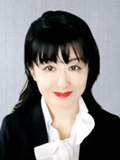
\includegraphics[width=.3\textwidth]{figure/facephoto.jpg} % 自分の顔写真(要らない場合はコメントアウトする)
  \end{center}
  \end{figure}
  }
  \vspace{20truept}
  {\huge 指導教員: 清水郁子 教授 \ }\\ % 指導教員名
  \vspace{10truept}
  {\normalsize 東京農工大学 工学部 知能情報システム工学科}\\
  \vspace{10truept}
  {\normalsize 20xx 年度卒業論文}\\
  \vspace{10truept}
  {\normalsize (20xx年 x月 x日 提出)}\\ % 提出日
  \end{center}
\end{titlepage}

\begin{titlepage}
  \newgeometry{left=20mm,right=20mm,bottom=30mm}
\begin{center}
{\normalsize 東京農工大学 工学部 知能情報システム工学科 20xx年度 卒業論文 要旨}\\
{\normalsize 題目 \ }
{\large ここに題目を書く}\\
{\normalsize You write your title here in English}\\
{\normalsize If your title is long, you write it here too.}\\
{\normalsize 学籍番号 00000000 \hspace{20pt}}
{\normalsize 氏名 自分野名前(Namae JIBUNNO)}\\
{\normalsize 提出日 20xx年 x月 x日}\\
\end{center}

ここに概要を書く.2000文字くらいで1ページ分.
概要には「背景」,「先行研究」,「目的」,「提案手法の内容」,「結果」を書く.
図は含めず,文章のみで説明する.

\restoregeometry
\end{titlepage}

%タイトル終わり
\frontmatter

\tableofcontents % 目次のリスト
\listoffigures % 図のリスト
\listoftables % 表のリスト

\mainmatter

\chapter{はじめに} % 章
\label{sec:はじめに}
\section{研究の背景}  % 節
\label{sec:研究の背景}

\section{本論文の構成}
\label{sec:本論文の構成}


\chapter{先行研究}\label{sec:RecentWorks}
本章では,先行研究で広く用いられるVision Transformer(ViT)について示したのち,それを用いたいくつかの先行研究を示す.

%%%%
\section{Vision Transformer}\label{sec:ViT}

研究の背景でもある Vision Transformer (ViT) \cite{Dosovitskiy_2021} は,
画像のクラス分類問題解決のために実装されたモデルである. 
モデルの設計は図 \ref{fig:vit_design} に示すとおりであり, 
Transformer Encoder \cite{Vaswani_2017} に BERT \cite{Devlin_2019} を適用した
``Transformer'' に加えて, 画像のトークン化を行う ``Tokenizer'' を構成要素に持つ. 
\begin{figure}[htbp]
  \centering
  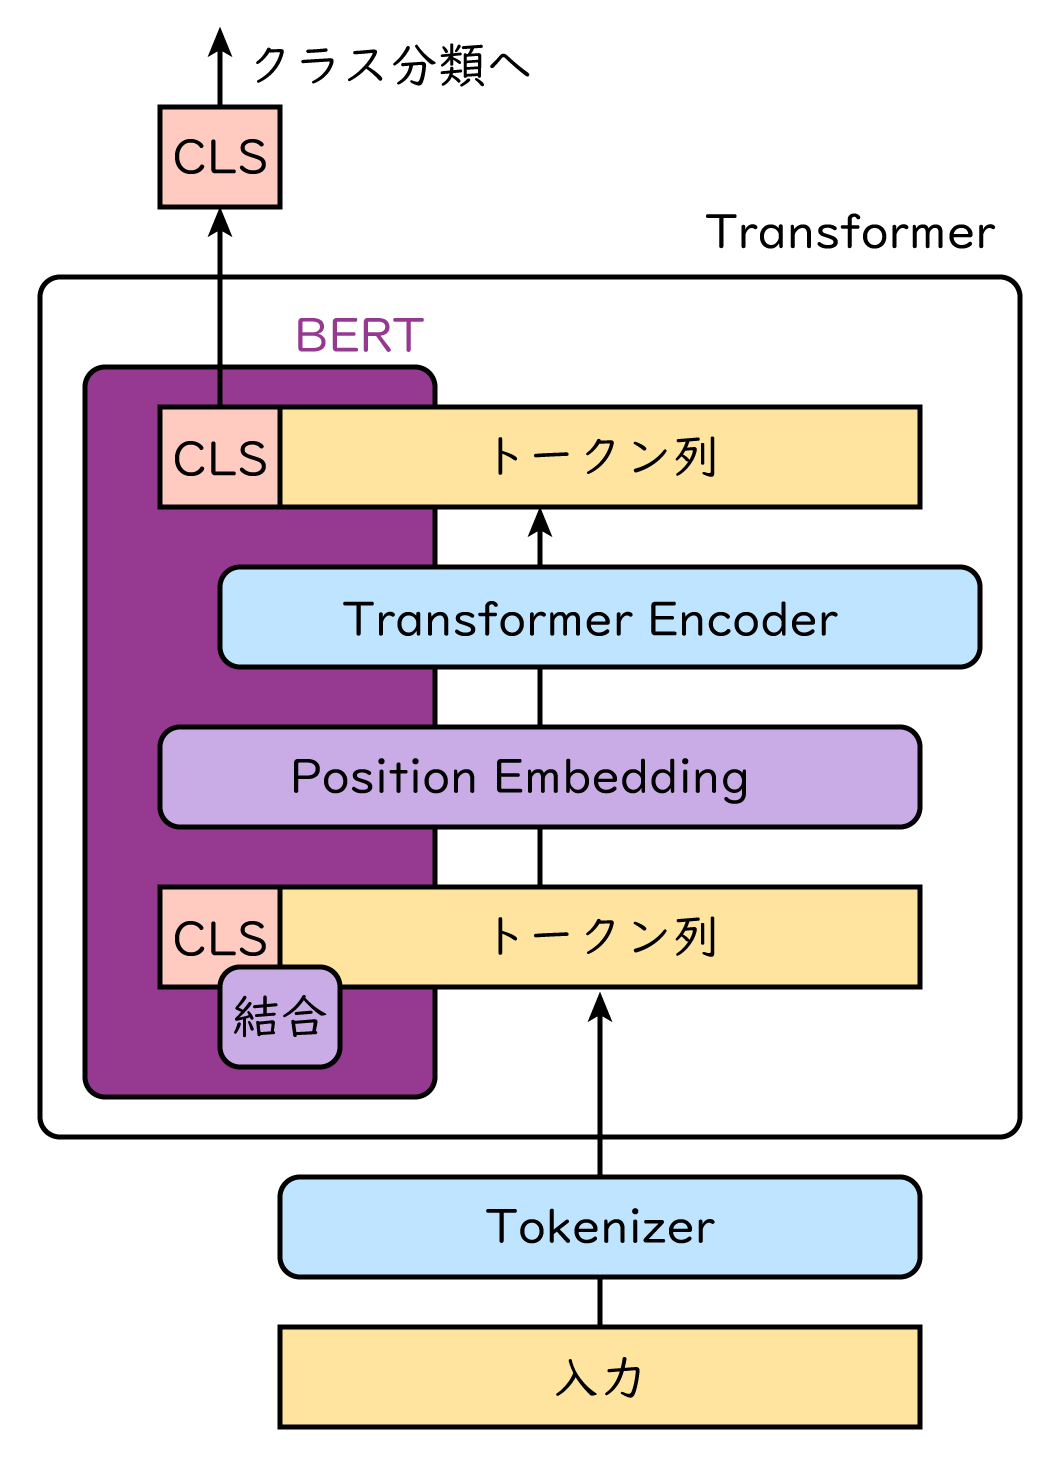
\includegraphics[width=.4\textwidth]{figure/vit_design.png}
  \caption{Vision Transformer の構成}
  \label{fig:vit_design}
\end{figure}

中略

%%%%
\subsection{BERT}\label{sec:bert}
BERT \cite{Devlin_2019} とは Bidirectional Encoder Representations from
Transformer の短縮表現であり, 自然言語処理領域にて発表されたモデルである.
ViT と同様, Transformer Encoder を基にしたモデルであり,
ViT の設計においても, BERTの要素技術が反映されている.

まず, ViTモデルのネットワーク規模は BERT の表現を踏まえたものとなっている.
具体的には, トークンの次元と Encoder Block の数, 次節で述べる MSA のヘッド数が
表 \ref{table:vit-netsize} のとおり定められている. 
ViT では Base(B) のネットワーク規模であることを, ViT-B と表記することで明示している. 
\begin{table}[htbp]
  \caption{ViT(BERT)のネットワーク規模}
  \label{table:vit-netsize}
  \centering
  \begin{tabular}{l|lccc}
    \hline
    ネットワーク規模 & ViTの表記 & トークンの次元($d_{t}$) & Encoder Block の数 
    & MSA のヘッド数 \\\hline\hline
    Base(B) & ViT-B & 768 & 12 & 12 \\
    Large(L) & ViT-L & 1024 & 24 & 16 \\
    \hline
  \end{tabular}
\end{table}

中略

%%%%
\subsection{計算量}\label{sec:calc}

トークン数 $l$ とその次元 $d_{t}$ による影響を明確にするため, 
$T \lparen d_{vec} \rparen$ は変数を用いた表現へと改める. 
内積における計算処理が, 要素積に対して総和を求めていることを考慮すると 
時間計算量 $T \lparen d_{vec} \rparen$ は $d_{vec}$ の比例関数とみなせるため, 
$\alpha d_{vec} + \beta$ によって近似する. 
加えて, ViT-B16においては, $d_{t}=hd_{m}=768$ かつ $l=256$ であるため, 
$ld_{t}$ および $l^{2}h$ は $ld_{t}^{2}$ や $l^{2}d_{t}$ に対して, 十分小さいものとする. 
以上から, 全体の時間計算量 $T_{msa}$ は式 \eqref{eq:cp_timesub} のとおり推定する.
時間計算量の推定値において, トークン数 $l$ による時間計算量のオーダーは 
$O \lparen n^{2} \rparen$ であり, トークン数の増加は実行時間に大きく影響することが分かる. 
\begin{align}
  \label{eq:cp_timesub}
  T_{msa} &= 3 l d_{t} \lparen \alpha d_{t} + \beta \rparen + l d_{t} \lparen \alpha d_{t} + \beta \rparen 
  + l^{2} h \lparen \alpha d_{m} + \beta \rparen + l d_{t} \lparen \alpha l + \beta \rparen \nonumber\\
  &= 2 l d_{t} \lparen 2 d_{t} + l \rparen \alpha  
\end{align} 
\chapter{提案手法}\label{sec:Method}
\section{提案手法の概要}\label{sec:AbstOfMethod}

\chapter{データセット}\label{sec:Dataset}
\chapter{実験}\label{sec:Experiments}
\include{acknowledgments} % 謝辞

\appendix
\chapter{補足} % 本文の補足 % 付録(つけない場合は\includeの部分ごとコメントアウトする)

\bibliographystyle{jplain} 
\bibliography{references} % 参考文献

\newpage
\printindex
\end{document}
